\section{Discussion}\label{sec:4-discussion}
The maintenance scheduling process effectively but not always efficiently models and 
determines good solutions to a complex scheduling
problem by relying on multiple actors. Through the use of actors the scheduling
process handles uncertainty that is difficult to reason about in a single
mathematical model. These  uncertainties are solved through coordination in
time (modelled as $\VarMetaTime$). Each type of actor in the process acts
according to a model each with different levels of aggregation and properties
where each actor has a solid understanding of his own model. In the discussion
interesting aspects of this approach has been divided into three 
sections: Section~\ref{sec:discussion:actors_and_integration}
actors and integration; Section~\ref{sec:discussion:continuous_optimization}
continuous optimization allows asynchronous optimization;  and
Section~\ref{sec:discussion:future_research} future research.

\subsection{Actors \& Integration}\label{sec:discussion:actors_and_integration}
Often in operation research the failure to reliably solve operational
problems in industry are not due to the problems being computationally
intractable \citep{gendreauHandbookMetaheuristics2019}. It is usually a practical
problem of connecting data streams so that the solution approach continually
receives dynamic data to handle changes and then sends the resulting
solutions to the relevant actors (stakeholders), ideally through a relevant interface
\citep{meignanReviewTaxonomyInteractive2015}. The actor-based approach proposed
in this paper makes integration easier by naturally encapsulating a model with a
reliable interface.

\subsection{Continuous Optimization}\label{sec:discussion:continuous_optimization}
With actor-based metaheuristics, the optimization loop can run indefinitely,
optimizing based on the latest available information. This may seem like a
detail as you could argue that you should only ever optimize the schedule
when there is an explicit need for it, but consider the case when you start
adding more than two actors to a scheduling system, then there arises a need
to coordinate people temporally as each will have to run their optimizing
process one after another. This is depicted in figure~\ref{fig:discussion:hierarchical_model_setup}
where the output of one model is used as the input to the next one, leading
to the hierarchical model setup.

\begin{figure}[H]
	\usetikzlibrary{positioning}
\usetikzlibrary{arrows.meta}
\usetikzlibrary{bending}
\definecolor{red}{HTML}{8A3F3A}
\definecolor{yellow}{HTML}{E0BB3C}
\definecolor{blue}{HTML}{4569E0}
\definecolor{green}{HTML}{17E561}
\definecolor{other}{HTML}{6A939E}

% DTU Colors
\definecolor{dtu-corporate-red}{HTML}{990000}
\definecolor{dtu-white}{HTML}{ffffff}
\definecolor{dtu-black}{HTML}{000000}
\definecolor{dtu-blue}{HTML}{2F3EEA}
\definecolor{dtu-bright-green}{HTML}{1FD082}
\definecolor{dtu-navy-blue}{HTML}{030F4F}
\definecolor{dtu-yellow}{HTML}{F6D04D}
\definecolor{dtu-orange}{HTML}{FC7634}
\definecolor{dtu-pink}{HTML}{F7BBB1}
\definecolor{dtu-grey}{HTML}{DADADA}
\definecolor{dtu-red}{HTML}{E83F48}
\definecolor{dtu-green}{HTML}{008835}
\definecolor{dtu-purple}{HTML}{79238E}


\newlength{\basisb}
\setlength{\basisb}{0.4cm}

\centering
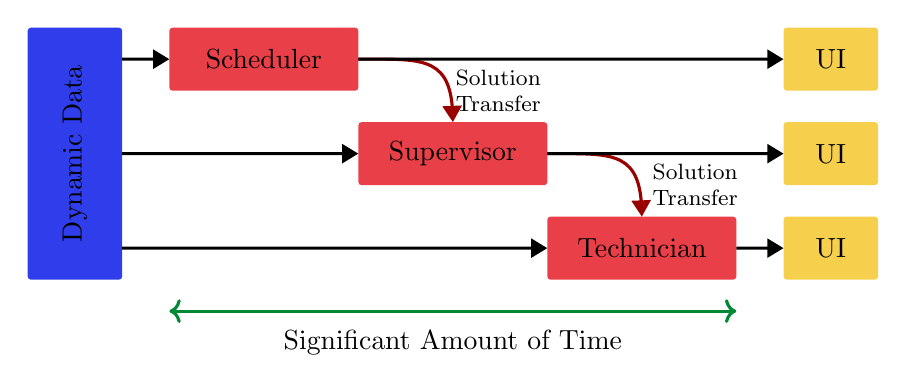
\begin{tikzpicture}[line width=0.0\basisb]
    \draw (2.0\basisb,4.0\basisb) 
		node[rotate=90, minimum height=3\basisb,fill=dtu-blue,minimum width=8\basisb,rounded corners=0.1\basisb] 
			(Dynamic Data) {Dynamic Data};

    \draw (8.0\basisb,7.0\basisb) 
		node[minimum height=2\basisb,fill=dtu-red,minimum width=6\basisb,rounded corners=0.1\basisb] 
			(Scheduler) {Scheduler};
    \draw (14.0\basisb,4.0\basisb) 
		node[minimum height=2\basisb,fill=dtu-red,minimum width=6\basisb,rounded corners=0.1\basisb] 
			(Supervisor) {Supervisor};
    \draw (20.0\basisb,1.0\basisb) 
		node[minimum height=2\basisb,fill=dtu-red,minimum width=6\basisb,rounded corners=0.1\basisb] 
			(Technician) {Technician};

    \draw (26.0\basisb,7.0\basisb) 
		node[minimum height=2\basisb,fill=dtu-yellow,minimum width=3\basisb,rounded corners=0.1\basisb] 
			(UserInterface1) {UI};
    \draw (26.0\basisb,4.0\basisb) 
		node[minimum height=2\basisb,fill=dtu-yellow,minimum width=3\basisb,rounded corners=0.1\basisb] 
			(UserInterface2) {UI};
    \draw (26.0\basisb,1.0\basisb) 
		node[minimum height=2\basisb,fill=dtu-yellow,minimum width=3\basisb,rounded corners=0.1\basisb] 
			(UserInterface3) {UI};

	\draw[<->, line width=0.1\basisb,color=dtu-green] (5.0\basisb, -1\basisb) -- (23.0\basisb, -1\basisb);
	\draw (14.0\basisb, -2.0\basisb) node {Significant Amount of Time};

	\draw[->,>=Triangle, thick, line width=0.1\basisb, color=dtu-corporate-red] (Scheduler) to[out=0, in=90,looseness=1.5]  (Supervisor);
	\draw[->,>=Triangle, thick, line width=0.1\basisb, color=dtu-corporate-red] (Supervisor) to[out=0, in=90,looseness=1.5] (Technician);
	\draw[->,>=Triangle, thick, line width=0.1\basisb] (Dynamic Data.south) ++(0\basisb,3.0\basisb) to[out=0, in=180,looseness=1.0] (Scheduler);
	\draw[->,>=Triangle, thick, line width=0.1\basisb] (Dynamic Data.south) to[out=0, in=180,looseness=1.0] (Supervisor);
	\draw[->,>=Triangle, thick, line width=0.1\basisb] (Dynamic Data.south) ++(0\basisb,-3.0\basisb) to[out=0, in=180,looseness=1.0] (Technician.west);
	\draw[<-,>=Triangle, thick, line width=0.1\basisb] (UserInterface1) to[out=180, in=0,looseness=1.0] (Scheduler);
	\draw[<-,>=Triangle, thick, line width=0.1\basisb] (UserInterface2) to[out=180, in=0,looseness=1.0] (Supervisor);
	\draw[<-,>=Triangle, thick, line width=0.1\basisb] (UserInterface3) to[out=180, in=0,looseness=1.0] (Technician);
	% \draw[<->, thick, line width=0.1\basisb] (Scheduler) -- (UserInterface);
	\begin{scope}[shift={(7,0)}] % Adjust shift to position the legend
    % Legend box
    % Legend lines and text
	    \draw[thick, line width=0.1\basisb] (-1.5,2.4) node[right, font=\footnotesize, align=center] {Solution\\Transfer};
	    \draw[thick, line width=0.1\basisb] (1.0,1.2) node[right, font=\footnotesize, align=center] {Solution\\Transfer};
	\end{scope}
\end{tikzpicture}
\label{fig:discussion:hierarchical_model_setup}
	\caption{Effects of using hierarchical models setups in human-guided search metaheuristics.
	Due to the dependent nature of each metaheuristic it becomes crucial that the running of 
	the metaheuristics are well coordinated between the actors.}
\end{figure}

In practice there are multiple problems with using a hierarchical setup.
Usually the biggest one is that the information and knowledge needed to 
execute a feasible schedule is usually found in the lower levels of the 
hierarchicy. The operational setting, where the
technicians are working, is usually so complex that it not feasible to 
centralize the knowledge that is required to create and execute a 
schedule. Figure~\ref{fig:discussion:asynchronous_setup}
shows the kind of non-hierarchical setup that an actor-based approach 
allows for.

\begin{figure}[H]
	\usetikzlibrary{positioning}
% \usetikzlibrary{arrows.meta}
\usetikzlibrary{bending}
\usetikzlibrary{backgrounds}
\definecolor{red}{HTML}{8A3F3A}
\definecolor{yellow}{HTML}{E0BB3C}
\definecolor{blue}{HTML}{4569E0}
\definecolor{green}{HTML}{17E561}
\definecolor{other}{HTML}{6A939E}

% DTU Colors
\definecolor{dtu-corporate-red}{HTML}{990000}
\definecolor{dtu-white}{HTML}{ffffff}
\definecolor{dtu-black}{HTML}{000000}
\definecolor{dtu-blue}{HTML}{2F3EEA}
\definecolor{dtu-bright-green}{HTML}{1FD082}
\definecolor{dtu-navy-blue}{HTML}{030F4F}
\definecolor{dtu-yellow}{HTML}{F6D04D}
\definecolor{dtu-orange}{HTML}{FC7634}
\definecolor{dtu-pink}{HTML}{F7BBB1}
\definecolor{dtu-grey}{HTML}{DADADA}
\definecolor{dtu-red}{HTML}{E83F48}
\definecolor{dtu-green}{HTML}{008835}
\definecolor{dtu-purple}{HTML}{79238E}


\newlength{\basisc}
\setlength{\basisc}{0.5cm}

\centering
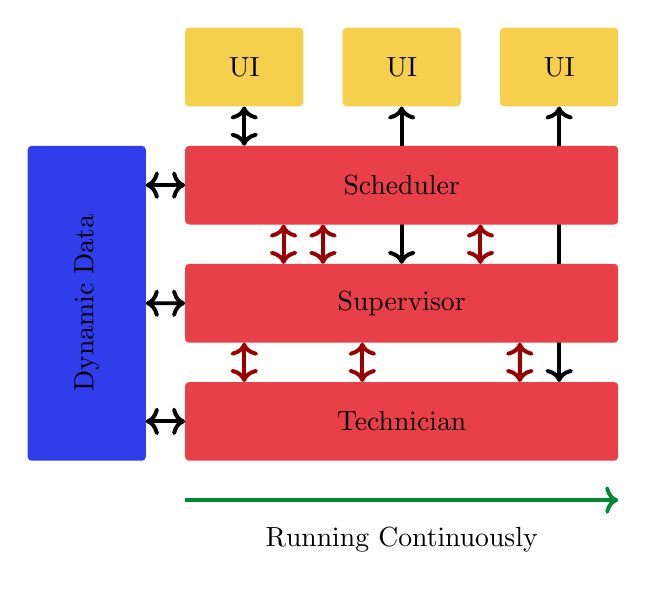
\begin{tikzpicture}[line width=0.0\basisc]
    \draw (4.0\basisc,4.0\basisc) 
		node[rotate=90, minimum height=3\basisc,fill=dtu-blue,minimum width=8\basisc,rounded corners=0.1\basisc] 
			(Dynamic Data) {Dynamic Data};

			

    \draw (8.0\basisc,10.0\basisc) 
		node[minimum height=2\basisc,fill=dtu-yellow,minimum width=3\basisc,rounded corners=0.1\basisc] 
			(UserInterface1) {UI};
    \draw (12.0\basisc,10.0\basisc) 
		node[minimum height=2\basisc,fill=dtu-yellow,minimum width=3\basisc,rounded corners=0.1\basisc] 
			(UserInterface2) {UI};
    \draw (16.0\basisc,10.0\basisc) 
		node[minimum height=2\basisc,fill=dtu-yellow,minimum width=3\basisc,rounded corners=0.1\basisc] 
			(UserInterface3) {UI};
    \draw (12.0\basisc,7.0\basisc) 
		node[minimum height=2\basisc,fill=dtu-red,minimum width=11\basisc,rounded corners=0.1\basisc] 
			(Scheduler) {Scheduler};
    \draw (12.0\basisc,4.0\basisc) 
		node[minimum height=2\basisc,fill=dtu-red,minimum width=11\basisc,rounded corners=0.1\basisc] 
			(Supervisor) {Supervisor};
    \draw (12.0\basisc,1.0\basisc) 
		node[minimum height=2\basisc,fill=dtu-red,minimum width=11\basisc,rounded corners=0.1\basisc] 
			(Technician) {Technician};


	\begin{pgfonlayer}{background}
		\draw[<->, thick, line width=0.1\basisc] (UserInterface1) to[out=-90, in=90,looseness=1.0] ++(0\basisc,-2.0\basisc)(Scheduler);
		\draw[<->, thick, line width=0.1\basisc] (UserInterface2) to[out=-90, in=90,looseness=1.0] (Supervisor);
		\draw[<->, thick, line width=0.1\basisc] (UserInterface3) to[out=-90, in=90,looseness=1.0] ++(0\basisc,-8.0\basisc)(Technician);

	\end{pgfonlayer}

	\draw[->, line width=0.1\basisc,color=dtu-green] (6.5\basisc, -1\basisc) -- (17.5\basisc, -1\basisc);
	\draw (12.0\basisc, -2.0\basisc) node {Running Continuously};

	\draw[<->, thick, line width=0.1\basisc, color=dtu-corporate-red] (Scheduler)++(-3\basisc, -1.0\basisc) to[out=-90, in=90,looseness=1.0]  ++(0\basisc, -1.0\basisc)(Supervisor);
	\draw[<->, thick, line width=0.1\basisc, color=dtu-corporate-red] (Scheduler)++(-2\basisc, -1.0\basisc) to[out=-90, in=90,looseness=1.0]  ++(0\basisc, -1.0\basisc)(Supervisor);
	\draw[<->, thick, line width=0.1\basisc, color=dtu-corporate-red] (Scheduler)++(2\basisc, -1.0\basisc) to[out=-90, in=90,looseness=1.0]  ++(0\basisc, -1.0\basisc)(Supervisor);

	\draw[<->, thick, line width=0.1\basisc, color=dtu-corporate-red] (Supervisor)++(-4\basisc, -1.0\basisc) to[out=-90, in=90,looseness=1.0] ++(0\basisc, -1.0\basisc)(Technician);
	\draw[<->, thick, line width=0.1\basisc, color=dtu-corporate-red] (Supervisor)++(-1\basisc, -1.0\basisc) to[out=-90, in=90,looseness=1.0] ++(0\basisc, -1.0\basisc)(Technician);
	\draw[<->, thick, line width=0.1\basisc, color=dtu-corporate-red] (Supervisor)++(3\basisc, -1.0\basisc) to[out=-90, in=90,looseness=1.0] ++(0\basisc, -1.0\basisc)(Technician);

	\draw[<->, thick, line width=0.1\basisc] (Dynamic Data.south) ++(0\basisc,3.0\basisc) to[out=0, in=180,looseness=1.0] (Scheduler);
	\draw[<->, thick, line width=0.1\basisc] (Dynamic Data.south) to[out=0, in=180,looseness=1.0] (Supervisor);
	\draw[<->, thick, line width=0.1\basisc] (Dynamic Data.south) ++(0\basisc,-3.0\basisc) to[out=0, in=180,looseness=1.0] (Technician.west);

	% \draw[<->, thick, line width=0.1\basisc] (Scheduler) -- (UserInterface);
\end{tikzpicture}

	\caption{Asynchronous model setup where each metaheuristic runs in perpetuity. In this setup
		there is no need to coordinate actors to run the metaheuristics. Each actor in the 
		scheduling process will always have the solutions of the other actors available to 
		him to guide his own search.
	}\label{fig:discussion:asynchronous_setup}
\end{figure}

When the optimization approach optimize continuously it enables tight
integration between the different model implementations. Instead of running
models to completion you simply handle changes in model parameters, model
solutions, user inputs, and in the dynamic data source as they occur opposed to
restarting the metaheuristics.

\subsection{Future Research}\label{sec:discussion:future_research}
The next step in this direction will be to model the remaining stakeholders as
their own  AbLNS metaheuristics, and then make them communicate together through
atomic pointer swaps and message passing. This enables modular concurrency at
each layer and ensures real-time synchronization across multiple optimization
levels. Making each metaheuristic expose solutions to each  other in real-time
providing each other with high quality parameters. 
Figure~\ref{fig:discussion:hexagon-setup} shows one such possible setup.


\begin{figure}[H]
	\usetikzlibrary {positioning}
\newcommand{\drawHexagon}[6][draw=black]{
	\draw[#1, fill=#4] (#2,#3) ++(30:#6) -- ++(90:#6) -- ++(150:#6) -- ++(210:#6) -- ++(270:#6) -- ++(330:#6) -- cycle;
	\node[align=center] at (#2,#3+2) {#5};
}

\newif\ifpersistencelayer
\newif\ifatomicpointerswaplayer
\newif\ifmetaheuristicslayer
\newif\ifuserinterfacelayer
\newif\iforchestratorlayer
\newif\ifsimplifiedlayer

\pgfkeys{
	/hexagon/.is family, /hexagon,
	default/.style = {
		persistence=false,
		atomicpointerswap=false,
		metaheuristics=false,
		orchestrator=false,
		userinterface=false,
		simplified=false,
	},
	persistence/.is if=persistencelayer,
	atomicpointerswap/.is if=atomicpointerswaplayer,
	metaheuristics/.is if=metaheuristicslayer,
	orchestrator/.is if=orchestratorlayer,
	userinterface/.is if=userinterfacelayer,
	simplified/.is if=simplifiedlayer,
}
\newcommand{\drawModelSetupHexagon}[1][]{
	\pgfkeys{/hexagon, default, #1}

	\begin{tikzpicture}[font=\footnotesize, scale=0.5, line width=1.05]
	

	\ifpersistencelayer
		\drawHexagon[draw=none]{ 2                      }{ 2}{dtu-blue}{}{2}
		\drawHexagon[draw=none]{{6 - 2 * (2 - sqrt(3)) }}{ 2}{dtu-blue}{}{2}
		\drawHexagon[draw=none]{{4 - 1 * (2 - sqrt(3)) }}{-1}{dtu-blue}{Persistence}{2}
		\drawHexagon[draw=none]{{0 + 1 * (2 - sqrt(3)) }}{-1}{dtu-blue}{}{2}
		\drawHexagon[draw=none]{{8 - 3 * (2 - sqrt(3)) }}{-1}{dtu-blue}{}{2}

		\drawHexagon[draw=none]{{2 - 0 * (2 - sqrt(3)) }}{-4}{dtu-blue}{}{2}
		\drawHexagon[draw=none]{{6 - 2 * (2 - sqrt(3)) }}{-4}{dtu-blue}{}{2}

		\drawHexagon[draw=none]{{10 - 4 * (2 - sqrt(3)) }}{-4}{dtu-blue}{}{2}
		\drawHexagon[draw=none]{{-2 + 2 * (2 - sqrt(3)) }}{-4}{dtu-blue}{}{2}

		\drawHexagon[draw=none]{{12 - 5 * (2 - sqrt(3)) }}{-1}{dtu-blue}{}{2}
		\drawHexagon[draw=none]{{-4 + 3 * (2 - sqrt(3)) }}{-1}{dtu-blue}{}{2}
		% Legend for each layer
		\drawHexagon{{14.0  }}{+3.0}{dtu-blue}{}{0.75}
		\node[align=right, anchor=west] at ({15.0}, +3.75) {Persistence};
		\drawHexagon{{14.0  }}{+1.5}{dtu-white}{}{0.75}
		\node[align=right, anchor=west] at ({15.0}, +2.25) {Atomic Pointer};
		\drawHexagon{{14.0  }}{+0.0}{dtu-white}{}{0.75}
		\node[align=right, anchor=west] at ({15.0}, +0.75) {Metaheuristics};
		\drawHexagon{{14.0  }}{-1.5}{dtu-white}{}{0.75}
		\node[align=right, anchor=west] at ({15.0}, -0.75) {Orchestration};
		\drawHexagon{{14.0  }}{-3.0}{dtu-white}{}{0.75}
		\node[align=right, anchor=west] at ({15.0}, -2.25) {User interfaces};
	\fi


	\ifatomicpointerswaplayer
		\drawHexagon[]{ 2                      }{ 2}{dtu-green}{Shared\\solution\\pointer}{2}
		\drawHexagon[]{{6 - 2 * (2 - sqrt(3)) }}{ 2}{dtu-green}{Shared\\solution\\pointer}{2}
		\drawHexagon[]{{4 - 1 * (2 - sqrt(3)) }}{-1}{dtu-green}{Shared\\solution\\pointer}{2}
		\drawHexagon[]{{0 + 1 * (2 - sqrt(3)) }}{-1}{dtu-green}{Shared\\solution\\pointer}{2}
		\drawHexagon[]{{8 - 3 * (2 - sqrt(3)) }}{-1}{dtu-green}{Shared\\solution\\pointer}{2}

		\drawHexagon[]{{2 - 0 * (2 - sqrt(3)) }}{-4}{dtu-green}{Shared\\solution\\pointer}{2}
		\drawHexagon[]{{6 - 2 * (2 - sqrt(3)) }}{-4}{dtu-green}{Shared\\solution\\pointer}{2}

		\drawHexagon[]{{10 - 4 * (2 - sqrt(3)) }}{-4}{dtu-green}{Shared\\solution\\pointer}{2}
		\drawHexagon[]{{-2 + 2 * (2 - sqrt(3)) }}{-4}{dtu-green}{Shared\\solution\\pointer}{2}

		\drawHexagon[]{{12 - 5 * (2 - sqrt(3)) }}{-1}{dtu-green}{Shared\\solution\\pointer}{2}
		\drawHexagon[]{{-4 + 3 * (2 - sqrt(3)) }}{-1}{dtu-green}{Shared\\solution\\pointer}{2}
		% Legend for each layer
		\drawHexagon{{14.0  }}{+3.0}{dtu-white}{}{0.75}
		\node[align=right, anchor=west] at ({15.0}, +3.75) {Persistence};
		\drawHexagon{{14.0  }}{+1.5}{dtu-green}{}{0.75}
		\node[align=right, anchor=west] at ({15.0}, +2.25) {Atomic Pointer};
		\drawHexagon{{14.0  }}{+0.0}{dtu-white}{}{0.75}
		\node[align=right, anchor=west] at ({15.0}, +0.75) {Metaheuristics};
		\drawHexagon{{14.0  }}{-1.5}{dtu-white}{}{0.75}
		\node[align=right, anchor=west] at ({15.0}, -0.75) {Orchestration};
		\drawHexagon{{14.0  }}{-3.0}{dtu-white}{}{0.75}
		\node[align=right, anchor=west] at ({15.0}, -2.25) {User interfaces};
	\fi

	\ifsimplifiedlayer

		\node[align=right, anchor=west] at ({-5.5}, +3.75) {};
		\drawHexagon{{+2 + 0 * (2 - sqrt(3)) }}{ 2}{dtu-green}{Scheduler}{2}
		\drawHexagon{{+4 - 1 * (2 - sqrt(3)) }}{-1}{dtu-red}{Supervisor}{2}
		\drawHexagon{{+0 + 1 * (2 - sqrt(3)) }}{-1}{dtu-red}{Supervisor}{2}
		\drawHexagon{{+2 - 0 * (2 - sqrt(3)) }}{-4}{dtu-corporate-red}{Technician}{2}
		\drawHexagon{{+6 - 2 * (2 - sqrt(3)) }}{-4}{dtu-corporate-red}{Technician}{2}
		\drawHexagon{{-2 + 2 * (2 - sqrt(3)) }}{-4}{dtu-corporate-red}{Technician}{2}
		\drawHexagon{{+8 - 3 * (2 - sqrt(3)) }}{-1}{dtu-corporate-red}{Technician}{2}
		\drawHexagon{{-4 + 3 * (2 - sqrt(3)) }}{-1}{dtu-corporate-red}{Technician}{2}

		% Scheduler
		\draw[thin, fill=dtu-yellow] (2, 5) circle (0.35);
		\draw[thin, fill=dtu-purple] (2, 3) circle (0.35);
		% Supervisor 1
		\draw[thin, fill=dtu-yellow] ({+4 - 1 * (2 - sqrt(3)) }, 02) circle (0.35);
		\draw[thin, fill=dtu-purple] ({+4 - 1 * (2 - sqrt(3)) }, -0) circle (0.35);
		% Supervisor 2
		\draw[thin, fill=dtu-yellow] ({+0 + 1 * (2 - sqrt(3)) }, 02) circle (0.35);
		\draw[thin, fill=dtu-purple] ({+0 + 1 * (2 - sqrt(3)) }, -0) circle (0.35);
		% Technician 1
		\draw[thin, fill=dtu-yellow] ({+2 - 0 * (2 - sqrt(3)) }, -1) circle (0.35);
		\draw[thin, fill=dtu-purple] ({+2 - 0 * (2 - sqrt(3)) }, -3) circle (0.35);
		% Technician 2
		\draw[thin, fill=dtu-yellow] ({+6 - 2 * (2 - sqrt(3)) }, -1) circle (0.35);
		\draw[thin, fill=dtu-purple] ({+6 - 2 * (2 - sqrt(3)) }, -3) circle (0.35);
		% Technician 3
		\draw[thin, fill=dtu-yellow] ({-2 + 2 * (2 - sqrt(3)) }, -1) circle (0.35);
		\draw[thin, fill=dtu-purple] ({-2 + 2 * (2 - sqrt(3)) }, -3) circle (0.35);
		% Technician 4
		\draw[thin, fill=dtu-yellow] ({+8 - 3 * (2 - sqrt(3)) }, 02) circle (0.35);
		\draw[thin, fill=dtu-purple] ({+8 - 3 * (2 - sqrt(3)) }, -0) circle (0.35);
		% Technician 5
		\draw[thin, fill=dtu-yellow] ({-4 + 3 * (2 - sqrt(3)) }, 02) circle (0.35);
		\draw[thin, fill=dtu-purple] ({-4 + 3 * (2 - sqrt(3)) }, -0) circle (0.35);

		% Legend for each layer
		\node[align=right, anchor=west] at ({12.0}, +3.75) {Atomic Pointer};
		\draw[fill=dtu-purple] (11.0,  +3.75) circle (0.5);

		\node[align=right, anchor=west] at ({12.0}, +2.25) {Scheduler Metaheuristic};
		\drawHexagon{{11.0  }}{+1.75}{dtu-green}{}{0.5}
		\node[align=right, anchor=west] at ({12.0}, +0.75) {Supervisor Metaheuristic};
		\drawHexagon{{11.0  }}{+0.25}{dtu-red}{}{0.5}
		\node[align=right, anchor=west] at ({12.0}, -0.75) {Technician Metaheuristic};
		\drawHexagon{{11.0  }}{-1.25}{dtu-corporate-red}{}{0.5}
		\node[align=right, anchor=west] at ({12.0}, -2.25) {User interfaces (Message Passing)};
		\draw[fill=dtu-yellow] (11.0, -2.25) circle (0.5);
	\fi

	\ifmetaheuristicslayer
		\drawHexagon{ 2                      }{ 2}{dtu-blue}{Strategic}{2}
		\drawHexagon{{6 - 2 * (2 - sqrt(3)) }}{ 2}{dtu-green}{Tactical}{2}
		\drawHexagon{{4 - 1 * (2 - sqrt(3)) }}{-1}{dtu-red}{Supervisor}{2}
		\drawHexagon{{0 + 1 * (2 - sqrt(3)) }}{-1}{dtu-red}{Supervisor}{2}
		\drawHexagon{{8 - 3 * (2 - sqrt(3)) }}{-1}{dtu-red}{Supervisor}{2}

		\drawHexagon{{2 - 0 * (2 - sqrt(3)) }}{-4}{dtu-corporate-red}{Technician}{2}
		\drawHexagon{{6 - 2 * (2 - sqrt(3)) }}{-4}{dtu-corporate-red}{Technician}{2}

		\drawHexagon{{10 - 4 * (2 - sqrt(3)) }}{-4}{dtu-corporate-red}{Technician}{2}
		\drawHexagon{{-2 + 2 * (2 - sqrt(3)) }}{-4}{dtu-corporate-red}{Technician}{2}

		\drawHexagon{{12 - 5 * (2 - sqrt(3)) }}{-1}{dtu-corporate-red}{Technician}{2}
		\drawHexagon{{-4 + 3 * (2 - sqrt(3)) }}{-1}{dtu-corporate-red}{Technician}{2}

		% Legend for each layer
		\drawHexagon{{14.0  }}{+3.0}{dtu-white}{}{0.75}
		\node[align=right, anchor=west] at ({15.0}, +3.75) {Persistence};
		\drawHexagon{{14.0  }}{+1.5}{dtu-white}{}{0.75}
		\node[align=right, anchor=west] at ({15.0}, +2.25) {Atomic Pointer};
		\drawHexagon{{14.0  }}{+0.0}{dtu-corporate-red}{}{0.75}
		\node[align=right, anchor=west] at ({15.0}, +0.75) {Metaheuristics};
		\drawHexagon{{14.0  }}{-1.5}{dtu-white}{}{0.75}
		\node[align=right, anchor=west] at ({15.0}, -0.75) {Orchestration};
		\drawHexagon{{14.0  }}{-3.0}{dtu-white}{}{0.75}
		\node[align=right, anchor=west] at ({15.0}, -2.25) {User interfaces};
	\fi

	\iforchestratorlayer
		\drawHexagon{ 2                      }{ 2}{dtu-orange}{}{2}
		\drawHexagon{{6 - 2 * (2 - sqrt(3)) }}{ 2}{dtu-orange}{}{2}
		\drawHexagon{{4 - 1 * (2 - sqrt(3)) }}{-1}{dtu-orange}{Orche-\\strator}{2}
		\drawHexagon{{0 + 1 * (2 - sqrt(3)) }}{-1}{dtu-orange}{}{2}
		\drawHexagon{{8 - 3 * (2 - sqrt(3)) }}{-1}{dtu-orange}{}{2}

		\drawHexagon{{2 - 0 * (2 - sqrt(3)) }}{-4}{dtu-orange}{}{2}
		\drawHexagon{{6 - 2 * (2 - sqrt(3)) }}{-4}{dtu-orange}{}{2}

		\drawHexagon{{10 - 4 * (2 - sqrt(3)) }}{-4}{dtu-orange}{}{2}
		\drawHexagon{{-2 + 2 * (2 - sqrt(3)) }}{-4}{dtu-orange}{}{2}

		\drawHexagon{{12 - 5 * (2 - sqrt(3)) }}{-1}{dtu-orange}{}{2}
		\drawHexagon{{-4 + 3 * (2 - sqrt(3)) }}{-1}{dtu-orange}{}{2}
		% Legend for each layer
		\drawHexagon{{14.0  }}{+3.0}{dtu-white}{}{0.75}
		\node[align=right, anchor=west] at ({15.0}, +3.75) {Persistence};
		\drawHexagon{{14.0  }}{+1.5}{dtu-white}{}{0.75}
		\node[align=right, anchor=west] at ({15.0}, +2.25) {Atomic Pointer};
		\drawHexagon{{14.0  }}{+0.0}{dtu-white}{}{0.75}
		\node[align=right, anchor=west] at ({15.0}, +0.75) {Metaheuristics};
		\drawHexagon{{14.0  }}{-1.5}{dtu-orange}{}{0.75}
		\node[align=right, anchor=west] at ({15.0}, -0.75) {Orchestration};
		\drawHexagon{{14.0  }}{-3.0}{dtu-white}{}{0.75}
		\node[align=right, anchor=west] at ({15.0}, -2.25) {User interfaces};
	\fi

	
	\ifuserinterfacelayer
		\drawHexagon{ 2                      }{ 2}{dtu-yellow}{UI}{2}
		\drawHexagon{{6 - 2 * (2 - sqrt(3)) }}{ 2}{dtu-yellow}{UI}{2}
		\drawHexagon{{4 - 1 * (2 - sqrt(3)) }}{-1}{dtu-yellow}{UI}{2}
		\drawHexagon{{0 + 1 * (2 - sqrt(3)) }}{-1}{dtu-yellow}{UI}{2}
		\drawHexagon{{8 - 3 * (2 - sqrt(3)) }}{-1}{dtu-yellow}{UI}{2}

		\drawHexagon{{2 - 0 * (2 - sqrt(3)) }}{-4}{dtu-yellow}{UI}{2}
		\drawHexagon{{6 - 2 * (2 - sqrt(3)) }}{-4}{dtu-yellow}{UI}{2}

		\drawHexagon{{10 - 4 * (2 - sqrt(3)) }}{-4}{dtu-yellow}{UI}{2}
		\drawHexagon{{-2 + 2 * (2 - sqrt(3)) }}{-4}{dtu-yellow}{UI}{2}

		\drawHexagon{{12 - 5 * (2 - sqrt(3)) }}{-1}{dtu-yellow}{UI}{2}
		\drawHexagon{{-4 + 3 * (2 - sqrt(3)) }}{-1}{dtu-yellow}{UI}{2}
		% Legend for each layer
		\drawHexagon{{14.0  }}{+3.0}{dtu-white}{}{0.75}
		\node[align=right, anchor=west] at ({15.0}, +3.75) {Persistence};
		\drawHexagon{{14.0  }}{+1.5}{dtu-white}{}{0.75}
		\node[align=right, anchor=west] at ({15.0}, +2.25) {Atomic Pointer};
		\drawHexagon{{14.0  }}{+0.0}{dtu-white}{}{0.75}
		\node[align=right, anchor=west] at ({15.0}, +0.75) {Metaheuristics};
		\drawHexagon{{14.0  }}{-1.5}{dtu-white}{}{0.75}
		\node[align=right, anchor=west] at ({15.0}, -0.75) {Orchestration};
		\drawHexagon{{14.0  }}{-3.0}{dtu-yellow}{}{0.75}
		\node[align=right, anchor=west] at ({15.0}, -2.25) {User interfaces};
	\fi
	
	\end{tikzpicture}
}

	\centering
	\resizebox{12cm}{!}{
		\drawModelSetupHexagon[simplified=true]
	}
	\caption{A software architecture tailored to metaheuristics (green and red)
		where solutions are shared between AbLNS algorithms in real-time through the
		use of atomic pointer swaps (purple). The messages in $m_{n}^{}(\tau)$ are
		inputted through userinterfaces (yellow)
	}\label{fig:discussion:hexagon-setup}
\end{figure}

Scaling metaheuristics is very difficult as metaheuristics are usually highly coupled
software components and this high coupling is exactly what enable them to optimize
a large system of equally coupled and nested decisions. The main contribution of 
future research will be to provide a shared memory software pattern that can be 
used to scale metaheuristics given metaheuristics unique architectual requirements.

\section{Conclusion}
Many current planning problems that industry faces are combinatorial by
nature, and many combinatorial problems have to be solved continuously to
make operations run efficiently. For operation research (OR) to be helpful
in this process, the solution methods should be a minimally invasive in the
workflow of the working stakeholders. The AbLNS solution approach detailed in
this paper aligns closely with two known problems in operation research: the
lack of integration and the issues of coordination in multi-actor processes.
For these reasons we argue that the ``standard'' Operations Research approach
of first collecting data, then creating a model and optimizing it, and then
finally providing the solution to the planners in the company workflow, is not a
scalable approach in many situations.

We have here demonstrated that the AbLNS approach works in a practical
maintenance scheduling setting at Total Energies. We believe that this approach
of combining a number of smaller planning/optimization problems with different
actors/stakeholders responsible for their part of the overall solution is the
future way of integrating Operation Research techniques in practice.

Modern industrial companies also have the available IT-infrastructure to support
and connect model/metaheuristics together with the relevant actors/stakeholders
in a way that was not possible just 10 years ago.

This also align with anacdotal evidence from practical operation research 
that smaller ``quick and dirty'' often works better in practice. 

The fundamental problem with the existing paradigm is that optimizing across
actors/stakeholders is very difficult, leading the literature to prefer
integrated models instead of decomposing the model by each of the
processes that make up a business process such as maintenance scheduling.
This paper argues that this is mainly due to an dated understanding of
software architecture that is available today in industry, but not
acknowledged by broader the Operations Research and Metaheuristic
communities \citep{talbiMetaheuristicsDesignImplementation2009},
\citep{gendreauHandbookMetaheuristics2019}.
